\documentclass{standalone}

\usepackage{tikz}
\usetikzlibrary{intersections,spath3,backgrounds}

\begin{document}

% Interstate shield framing
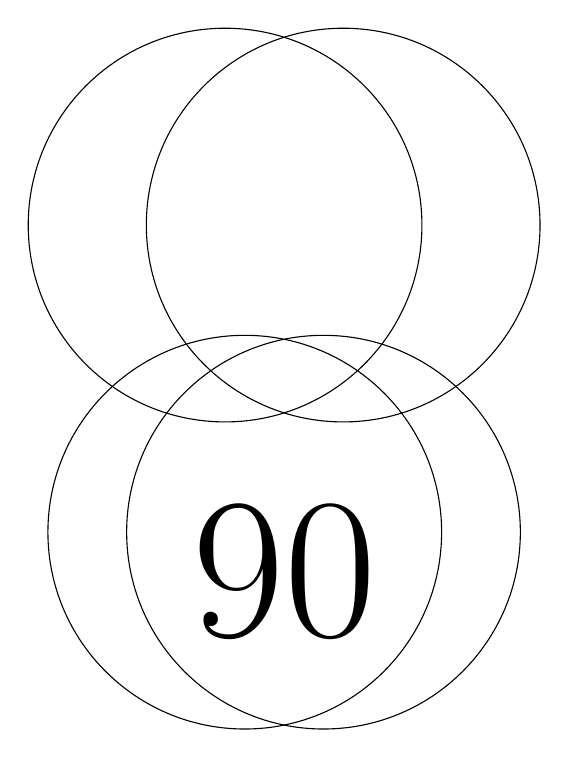
\begin{tikzpicture}
  \foreach\i in {-1,1}
  {
    \draw (0.5*\i,0.5) circle (2.5);
    \draw (0.75*\i,4.4) circle (2.5);
  }
\node[scale =3.5] at (0,0) {\huge 90};
\end{tikzpicture}


\begin{tikzpicture}[framed]
  \useasboundingbox (-2,-2) rectangle (2,2);
  % framing
  \path[spath/save=circleBL] (-0.5,0.5) circle (2.5);
  \path[spath/save=circleBR] (0.5,0.5) circle (2.5);
  \path[spath/save=circleTL] (-0.75,4.4) circle (2.5);
  \path[spath/save=circleTR] (0.75,4.4) circle (2.5);
  % spath3 operations
  \tikzset
  {% cutting
    spath/split at intersections={circleBL}{circleBR},
    spath/split at intersections={circleBL}{circleTR},
    spath/split at intersections={circleBR}{circleTL},
    spath/split at intersections={circleTL}{circleTR},
    % store the pieces
    spath/get components of={circleBL}\cBL,
    spath/get components of={circleBR}\cBR,
    spath/get components of={circleTL}\cTL,
    spath/get components of={circleTR}\cTR,
  }
  % shield
  \draw[
    spath/use=\getComponentOf\cBL{4},
    spath/use={\getComponentOf\cTR{3},reverse,weld},
    spath/use={\getComponentOf\cTL{2},reverse,weld},
    spath/use={\getComponentOf\cBR{3},weld},
  ];
  \node[scale =3.5] at (0,0) {\huge 90};
\end{tikzpicture}

% Generic highway shield framing
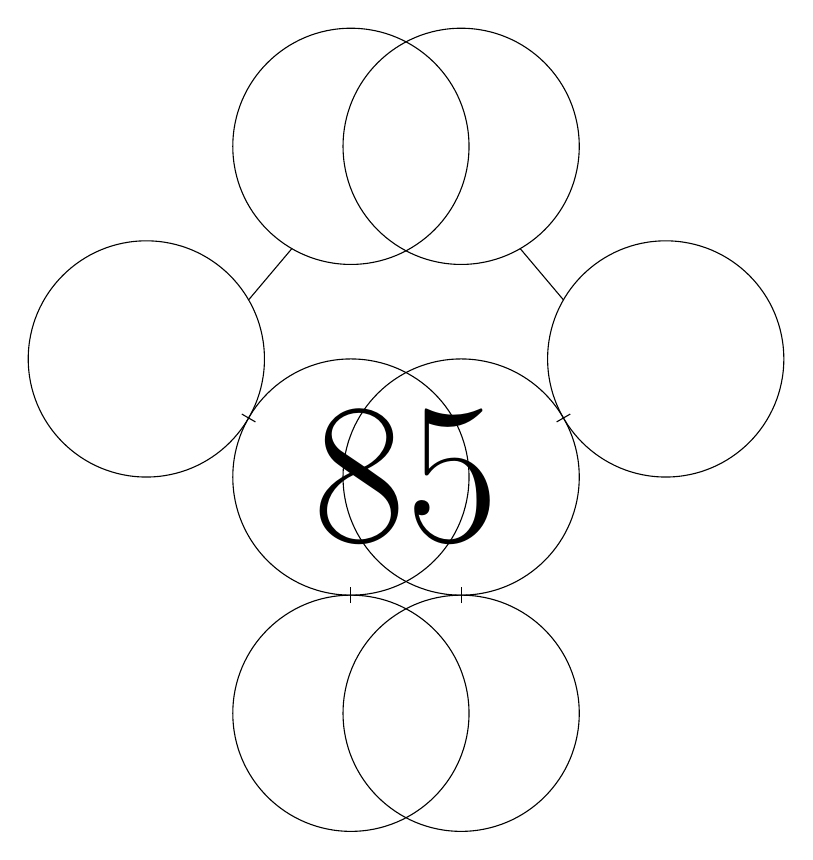
\begin{tikzpicture}
  \foreach\i in {-1,1}
  {
    % top
    \draw (0.7*\i,4.2) circle (1.5);
    % center
    \draw (0.7*\i,0) circle (1.5);
    % top-center-outside
    \draw ({(sqrt(3)/2*3+0.7)*\i},1.5) circle (1.5); 
    % bottom
    \draw (0.7*\i,-3) circle (1.5);
    % connecting top and top-center-outside
    \draw (({(0.7+0.5*1.5)*\i},{4.2-sqrt(3)/2*1.5}) --
    ({(sqrt(3)/2*3+0.7-sqrt(3)/2*1.5)*\i},{1.5+0.5*1.5});
    % nodes to exaggerate tangent circles...
    \draw (0.7*\i,-1.6) -- (0.7*\i,-1.4);
    \draw ({(0.7+1.4*sqrt(3)/2)*\i},1.4*0.5) -- ({(0.7+1.6*sqrt(3)/2)*\i},1.6*0.5);
  }
\node[scale =3.5] at (0,0) {\huge 85};
\end{tikzpicture}


\begin{tikzpicture}[framed]
  \useasboundingbox (-2.2,-1.8) rectangle (2.2,2.9);
  % framing
  \path[spath/save=circleTL] (-0.7,4.2) circle (1.5);
  \path[spath/save=circleTR] (0.7,4.2) circle (1.5);
  \path[spath/save=circleCL] (-0.7,0) circle (1.5);
  \path[spath/save=circleCR] (0.7,0) circle (1.5);
  \path[spath/save=circleTCL] ({-(sqrt(3)/2*3+0.7)},1.5) circle (1.5);
  \path[spath/save=circleTCR] ({(sqrt(3)/2*3+0.7)},1.5) circle (1.5);
  \path[spath/save=circleBL] (-0.7,-3) circle (1.5);
  \path[spath/save=circleBR] (0.7,-3) circle (1.5);
  \path[spath/save=connectorTL] (({-(0.7+0.5*1.5)},{4.2-sqrt(3)/2*1.5}) -- ({-(sqrt(3)/2*3+0.7-sqrt(3)/2*1.5)},{1.5+0.5*1.5});
  \path[spath/save=connectorTR] (({(0.7+0.5*1.5)},{4.2-sqrt(3)/2*1.5}) -- ({(sqrt(3)/2*3+0.7-sqrt(3)/2*1.5)},{1.5+0.5*1.5});
  \path[spath/save=splitterTL] ({-(0.7+1.4*sqrt(3)/2)},1.4*0.5) -- ({-(0.7+1.6*sqrt(3)/2)},1.6*0.5);
  \path[spath/save=splitterTR] ({0.7+1.4*sqrt(3)/2},1.4*0.5) -- ({0.7+1.6*sqrt(3)/2},1.6*0.5);
  \path[spath/save=splitterBL] (-0.7,-1.6) -- (-0.7,-1.4);
  \path[spath/save=splitterBR] (0.7,-1.6) -- (0.7,-1.4);
  % spath3 operations
  \tikzset
  {% cutting
    spath/split at intersections={circleTL}{circleTR},
    spath/split at intersections with={circleTL}{connectorTL},
    spath/split at intersections with={circleTCL}{connectorTL},
    spath/split at intersections with={circleTCL}{splitterTL},
    spath/split at intersections with={circleCL}{splitterTL},
    spath/split at intersections with={circleCL}{splitterBL},
    spath/split at intersections with={circleBL}{splitterBL},
    spath/split at intersections={circleBL}{circleBR},
    spath/split at intersections with={circleBR}{splitterBR},
    spath/split at intersections with={circleCR}{splitterBR},
    spath/split at intersections with={circleCR}{splitterTR},
    spath/split at intersections with={circleTCR}{splitterTR},
    spath/split at intersections with={circleTCR}{connectorTR},
    spath/split at intersections with={circleTR}{connectorTR},
    % store the pieces
    spath/get components of={circleTL}\cTL,
    spath/get components of={circleTR}\cTR,
    spath/get components of={circleTCL}\cTCL,
    spath/get components of={circleTCR}\cTCR,
    spath/get components of={circleCL}\cCL,
    spath/get components of={circleCR}\cCR,
    spath/get components of={circleBL}\cBL,
    spath/get components of={circleBR}\cBR,
    spath/get components of={connectorTL}\connTL,
    spath/get components of={connectorTR}\connTR,
  }

  % shield
  \draw[
    spath/use={\getComponentOf\cTR{3}},
    spath/use={\getComponentOf\connTR{1},weld},
    spath/use={\getComponentOf\cTCR{3},weld},
    spath/use={\getComponentOf\cCR{2},reverse,weld},
    spath/use={\getComponentOf\cBR{4},weld},
    spath/use={\getComponentOf\cBL{4},weld},
    spath/use={\getComponentOf\cCL{2},reverse,weld},
    spath/use={\getComponentOf\cTCL{3},weld},
    spath/use={\getComponentOf\connTL{1},reverse,weld},
    spath/use={\getComponentOf\cTL{3},weld},
  ];
  \node[scale =3.5] at (0,0) {\huge 85};
\end{tikzpicture}

\end{document}
